% Файзиев Фаридун Равшанович - P3112 - 2022г
% Вариант - 37
% https://kvant.ras.ru/1973/07/poverhnostnoe_natyazhenie.htm
\documentclass{article}
\usepackage[utf8]{inputenc}
\usepackage[russian]{babel}
\usepackage{multicol, caption}
\usepackage{graphicx}
\usepackage{fancyhdr}
\usepackage[dvipsnames]{xcolor}
\usepackage{colortbl}
\usepackage{amsmath}
\usepackage{setspace}
\usepackage[left=10mm, top=-1mm, right=10mm, bottom=10mm, nohead, nofoot]{geometry}
\captionsetup{justification   = raggedright, % Номер рисунков на лево
              singlelinecheck = false}
      

\pagestyle{fancy}
\fancyhf{}
\fancyfoot[R]{11}
\pagecolor{Apricot}

\begin{document}

\noindent\makebox[\linewidth]{\rule{21cm}{0.4pt}}
\begin{multicols}{3}
\begin{flushright}
\vspace*{\fill}
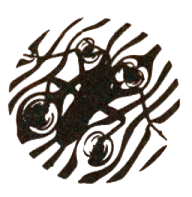
\includegraphics[scale=0.5]{title.png}
\vspace*{\fill}
\end{flushright}
\vspace*{\fill}
\begin{flushleft}
\Huge
\textbf{Поверхностное натяжение}\\
\Large
\textit{Л. Г. Асламазов}    
\end{flushleft}
\vspace*{\fill}
\end{multicols}
\noindent\makebox[\linewidth]{\rule{21cm}{0.4pt}}

\setlength{\columnsep}{30pt}
\begin{multicols}{2}
\large
\noindentУдивительно разнообразны проявле-\linebreak
ния поверхностного натяжения жид-\linebreak
костей в природе и технике. Оно со-\linebreak
бирает воду В капли, благодаря ему\linebreak
мы можем выдуть мыльный пузырь\linebreak
и писать ручкой. Поверхностное на-\linebreak
тяжение играет важную роль в физио-\linebreak
логии нашего организма. Его исполь-\linebreak
зуют в космической технике. Почему\linebreak
же поверхность жидкости ведет себя\linebreak
подобно растянутой упругой пленке?\linebreak
Попробуем в этом разобраться. \\ \\
\large
\textbf{Поверхностная энергия}\\
\large
Молекулы, расположенные в тонком\linebreak
слое жидкости вблизи поверхности,\linebreak
находятся в особых условиях. Они\linebreak
имеют одинаковых с ними соседей\linebreak
только с одной стороны поверхности;\linebreak
в отличие от молекул внутри жид-\linebreak
кости, окруженных ‘со всех сторон\linebreak
такими же молекулами. Поэтому ре-\linebreak
зультирующая сила, действующая на\linebreak
молекулу в поверхностном слое, от-\linebreak
‚лична от нуля. Например, на свобод-\linebreak
ной поверхности жидкости (рис. 1)\ref{ris:image}\linebreak
эта сила направлена внутрь жидкос-


\begin{Figure}
 \centering
  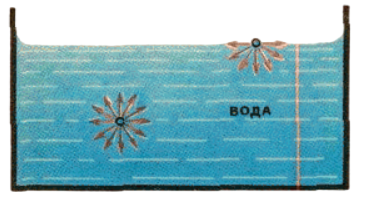
\includegraphics[width=\linewidth]{pic1.png}
  \begin{flushright}
   \captionof{figure}{}
  \end{flushright}
  \label{ris:image}
\end{Figure}

\large
\noindent
ти, так как молекула на поверхности\linebreak
испытывает значительно большее\linebreak
притяжение со стороны молекул\linebreak
жидкости, чем со стороны молекул\linebreak
воздуха.

При перемещении молекулы с по-\linebreak
верхности в объем жидкости совер-\linebreak
шается положительная работа. Это\linebreak
означает, что молекулы в поверхност-\linebreak
ном слое обладают избыточной потен-\linebreak
циальной энергией по сравнению с\linebreak
молекулами внутри жидкости. Разу-\linebreak
меется, молекулы жидкости находят-\linebreak
ся в непрерывном тепловом движе-\linebreak
нии — одни молекулы уходят с по-\linebreak
верхности, другие, наоборот, попадают\linebreak
на нее. Но можно говорить о средней\linebreak
добавочной энергии поверхностного\linebreak
слоя жидкости — о поверхностной\linebreak
энергии, пропорциональной площади\linebreak
поверхности жидкости.

Известно, что из всех возможных\linebreak
состояний системы устойчивым явля-\linebreak
ется то, в котором энергия системы\linebreak
минимальна, В частности, и поверх-\linebreak
ность жидкости ‘стремится принять\linebreak
такую форму, при которой ее поверх-\linebreak
ностная энергия будет минимальна.\linebreak
Как говорят, жидкость обладает по-\linebreak
верхностным натяжением, стремящим-\linebreak
ся сократить, уменьшить ее поверх-\linebreak
ность. Коэффициентом поверхностного\linebreak
натяжения называют поверхностную\linebreak
энергию, приходящуюся на единицу\linebreak
площади, или силу, приходящуюся\linebreak
на единицу длины границы поверх-\linebreak
ности. Легко доказать (сделайте это\linebreak
сами), что оба определения коэффи-\linebreak
циента поверхностного натяжения эк-\linebreak
вивалентны.

\end{multicols}

\newpage
\renewcommand{\headrulewidth}{0pt}
\newgeometry{left=2cm,right=2cm,top=2cm,bottom=3cm}
\pagestyle{fancy}
\fancyhf{}
\nopagecolor
\linespread{2}
\begin{center}
\Large
\textbf{Формулы:} \\
$\sqrt{x^2+1}$ \\
$\sqrt[n]{1+x+x^2+x^3+\dots+x^n}$ \\
$\cos (2\theta) = \cos^2 \theta - \sin^2 \theta$ \\
$f(n) = n^5 + 4n^2 + 2 |_{n=17}$ \\
$k_{n+1} = n^2 + k_n^2 - k_{n-1}$ \\
$\frac{n!}{k!(n-k)!} = \binom{n}{k}$ \\
$\sum_{i=1}^{10} t_i$ \\
$\int_0^\infty \mathrm{e}^{-x}\,\mathrm{d}x$ \\

\Large
\textbf{Основные единицы:}\\

\begin{tabular}[b]{ | m{0.3cm} | m{2.8cm} | m{2.5cm} | m{1.6cm}  | }
\hline
\text{1} & \text{Длина} & \text{сантиметр} & \text{см} \\
\hline
\text{2} & \text{Масса} & \text{грамм} & \text{г} \\
\hline
\text{3} & \text{Время} & \text{секунда} & \text{с} \\
\hline
\text{4} & \text{Сила} & \text{дина} & \text{дин} \\
\hline
\end{tabular}
\end{center}


\end{document}
